Czy chcesz, żeby Twoja praca dyplomowa wyglądała porządnie, schludnie a~może nawet profesjonalnie? Nie masz ochoty męczyć się z~ręcznym formatowaniem kilkudziesięciu stron tekstu i~pilnowaniem, by wszystkie akapity wyglądały tak samo?

Jeśli tak, to użyj niniejszego szablonu pracy dyplomowej! Działa on dla prac inżynierskich i~magisterskich na Wydziale Elektrycznym, również na studiach anglojęzycznych -- wystarczy zmienić jedną wartość w~pliku głównym, czyli \href{./EE-dyplom.tex}{EE-dyplom.tex}. Jeśli nie wiesz jak zacząć korzystanie z~\LaTeX{a} to możesz znaleźć interesujący Cię fragment, skopiować go do swojej pracy i~zmodyfikować. Nic trudnego, na pewno dasz radę! Powodzenia!

W niniejszym przykładzie znajdują się zastosowane w~praktyce takie elementy \LaTeX{a} jak:
\begin{itemize}
    \item podział tekstu na rozdziały, podrozdziały i~akapity
    \item przypisy dolne,
    \item wstawianie rysunków,
    \item odwołania do rysunków w~tekście,
    \item cytaty i~odwołania do bibliografii,
    \item wypunktowania, takie jak na przykład niniejsze,
    \item użycie kolorów dla tekstu,
    \item tabele, w~tym tabele kolorowane, % TODO
    \item wzory, % TODO
    \item wstawianie kodów źródłowych.
\end{itemize}

Każdy rozdział zaczyna się od tekstu\footnote{Niepoprawne jest na przykład rozpoczęcie podrozdziału (,,section'') zaraz po rozpoczęciu rozdziału (,,chapter'') bez tekstu między nimi.}.

Pusta linia oznacza nowy akapit.
Ta linia kontynuuje poprzedni akapit, chociaż w~edytorze jest odrębną linią, oddzieloną ,,enterem''.

To będzie nowy akapit. Będzie miał wcięcie. Tylko pierwszy akapit, zaraz po tytule rozdziału albo śródtytule -- nie ma wcięcia i~jest to prawidłowe podejście do składu tekstu. Możesz to zobaczyć na niniejszej stronie.

%%%%%%%%%%%%%%%%%%%%%%%%%%%%%%%%%%%%%%%%%%%%%%%%
\section{Rysunki}
Rysunki w~\LaTeX{u} wstawiane są za pomocą \texttt{includegraphics}. Tego polecenia najczęściej używa się w~otoczeniu \texttt{figure}, które pozwala na dodanie podpisu (\texttt{caption}) i~znacznika (\texttt{label}), dzięki któremu można się później do tego rysunku odwołać za pomocą \texttt{ref}. Nowo dodany znacznik wymaga dwukrotnego uruchomienia kompilacji, gdyż za pierwszym razem \LaTeX{} zauważa go a~za drugim już wie, dokąd mają prowadzić i~gdzie umieszczać odniesienia.

Przykładem jest rysunek~\ref{rys:kopernik}, przedstawiający portret wybitnego polskiego astronoma -- Mikołaja Kopernika. W~tym przykładzie szerokość grafiki z~portretem astronoma jest ustawiona na dokładnie 0,618 szerokości linii tekstu. Praca wygląda dobrze, jeśli szerokości rysunków są powtarzalne, wybierane spośród tylko 2 lub 3 wartości. Niniejszy, przykładowy dokument celowo używa różnych wartości i~metod określania wymiarów rysunków.

\begin{figure}[!hb]
	\centering 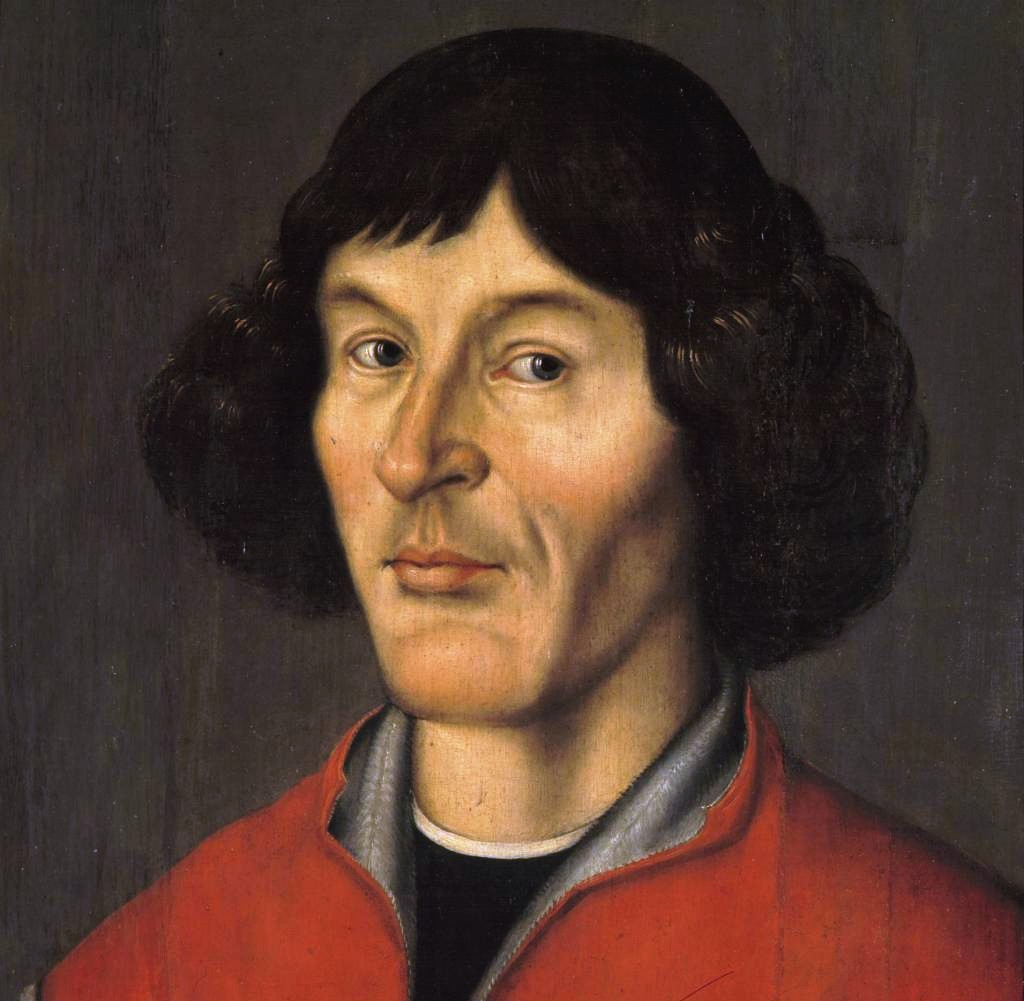
\includegraphics[width=0.618\linewidth]{Kopernik.jpg} % rysunek o szerokości 0.618 długości linii tekstu - złoty podział
	\caption{Mikołaj Kopernik, autor nieznany, r. 1580}
	\label{rys:kopernik}
\end{figure}

\begin{figure}
\centering
\begin{subfigure}{.5\textwidth}
  \centering
  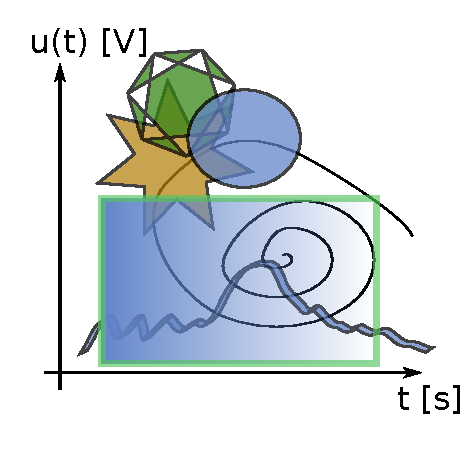
\includegraphics[width=.99\linewidth]{wektorowo.pdf} % rysunek niemal na szerokość linii ale w ramach "subfigure"
  \caption{Rysunek wektorowy}
  \label{rys:wektorowopdf}
\end{subfigure}%
\begin{subfigure}{.5\textwidth}
  \centering
  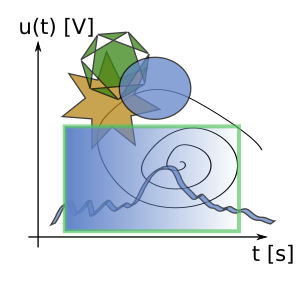
\includegraphics[width=.99\linewidth]{wektorowo.png}
  \caption{Rysunek rastrowy}
  \label{rys:wektorowopng}
\end{subfigure}
\caption{Porównanie rysunku wektorowego i~rastrowego}
\label{rys:wektorowo}
\end{figure}

Istotną kwestią rysunków technicznych jest ich jakość. Jakość rysunków rastrowych jest ograniczona ich rozdzielczością mierzoną liczbą punktów (pikseli) na daną jednostkę długości. Dobry wydruk rastrowy to przynajmniej 600 dpi czyli punktów na cal. Można uzyskać ,,nieskończoną'' rozdzielczość stosując grafikę wektorową.

Na rysunku~\ref{rys:wektorowo} widzimy porównanie efektu użycia grafiki wektorowej i~rastrowej. Obrazek po lewej stronie jest samodzielnym plikiem PDF, który wykorzystuje grafikę wektorową. Obrazek po prawej stronie to wersja wyeksportowana do pliku PNG, skompresowanego bezstratnie. Po powiększeniu podglądu widzimy na rysunku~\ref{rys:wektorowopdf} gładkie linie w~przeciwieństwie do rysunku~\ref{rys:wektorowopng} gdzie dostrzeżemy pojedyncze piksele. Efekt ten nie musi być łatwy do zauważenia na ekranie komputera, który typowo ma rozdzielczość około 100 ppi (pikseli na cal) a~czasami zaledwie 72 ppi. Jednak problem ten ujawni się po wydrukowaniu pracy.

Rysunek na pewno powinien znajdować się w~obrębie rozdziału lub podrozdziału, który ten rysunek opisuje. O rysunku nie należy myśleć w~kontekście umieszczenia go powyżej lub poniżej odwołania w~tekście. Rysunek ma trafić w~takie miejsce, by czytelnik mógł go od razu spostrzec, gdy w~tekście pojawia się odwołanie do tego rysunku. Tutaj, niestety w~przypadku rysunku~\ref{rys:wektorowo} się to nie udało. Czytelnik będzie musiał obrócić stronę. Czasem to jedyna możliwość, bez dopisania dodatkowego tekstu, który ,,przepchnie'' odwołanie do rysunku lub sam rysunek w~inne miejsce.

Jeśli rysunek nie trafia Twoim zdaniem tam, gdzie powinien, to spróbuj przenieść go poniżej lub powyżej sąsiadujących akapitów. Możesz też zmienić wartość ,,!hb'' (ang. \textit{here or bottom}) na ,,!ht'' (ang. \textit{here or top}) i~na odwrót lub na tylko jedną z~liter określających posadowienie rysunku. Wykrzyknik oznacza przymuszenie \LaTeX{a} by nie ,,uciekł'' z~rysunkiem na koniec rozdziału.

Zazwyczaj problemy z~ulokowaniem rysunku wynikają z~tego, że otaczającej go treści jest zbyt mało, w~porównaniu z~powierzchnią zajmowaną przez ten rysunek. Dlatego ostateczne rozlokowanie rysunków najlepiej odłożyć na koniec pisania pracy i~wtedy też można ustalić pożądaną wielkość rysunków.

W~\LaTeX{u} praktycznie nie ma ryzyka, że wszystko ,,się rozjedzie'', gdy przesuniemy rysunek. Ewentualne zmiany znacznie łatwiej cofnąć, niż w~typowych edytorach tekstu.

%%%%%%%%%%%%%%%%%%%%%%%%%%%%%%%%%%%%%%%%%%%%%%%%
\section{Odniesienia do literatury}
Zarządzanie bibliografią w~\LaTeX{u} odbywa się w~sposób zautomatyzowany. Nie ma problemu z~dodaniem lub usunięciem pozycji bibliograficznej, kolejnością pozycji listy literatury i~spójnością między odwołaniami w~treści a~listą pozycji bibliograficznych. O tego rodzaju trudnościach, znanych z~innych programów, można tu zapomnieć.

Odniesienia do literatury robi się za pomocą polecenia \texttt{cite}. W~argumencie tego polecenia podaje się znacznik przypisany danej pozycji literaturowej a~nie konkretny numer. Przekształceniem znaczników na konkretne numery zajmuje się \LaTeX{}. Noty bibliograficzne z~ich znacznikami muszą znajdować się w~osobnym pliku \href{./EE-dyplom.bib}{EE-dyplom.bib}. Każda zmiana pliku z~bibliografią wymaga jego rekompilacji. W~tym szablonie stosowany jest program Biber (z linii poleceń: \texttt{biber}), który w~Overleaf jest uruchamiany automatycznie po wykryciu zmian w~pliku bibliografii.

Niniejszy szablon zawiera przykładowe noty bibliograficzne różnorodnych typów literatury. Do realizacji pracy dyplomowej będą przydatne przede wszystkim deklaracje:
\begin{itemize}
    \item artykułów z~czasopism naukowych,
    \item artykułów z~konferencji,
    \item książek,
    \item dokumentów technicznych.
\end{itemize}

Oto przykładowe odwołanie do literatury~\cite{fowler2009}. Wszystkie odwołania robi się praktycznie tak samo. Chcąc odnieść się do kilku pozycji jednocześnie, trzeba ich znaczniki wpisać po przecinku~\cite{maxwell1865,leksinski1995}. Można też odnieść się do konkretnej strony~\cite[s.~38]{leksinski1995}. Znak tyldy przed wywołaniem \texttt{cite} ,,skleja'' odnośnik z~poprzedzającym je słowem za pomocą tak zwanej ,,twardej'' spacji.

Do spisu literatury znajdującego się pod koniec pracy dyplomowej trafią tylko te pozycje, dla których w~tekście znajduje się odwołanie zrobione za pomocą \texttt{cite}. Dzięki temu można łatwo dodać sobie literaturę ,,na potem'' a~decyzję o~skorzystaniu z~niej podjąć później. Można też usunąć odniesienie do literatury z~tekstu pracy i~nie przejmować się tym, że dana pozycja nadal jest obecna w~pliku bibliograficznym. 

Literatura jest sortowana automatycznie po nazwiskach autorów, co jest zgodne z~obowiązującymi na PW zaleceniami. Dlatego w~wynikowym tekście oznaczenia numeryczne pojawią się w~przypadkowej kolejności i~jest to prawidłowe. Kolejność wpisów w~pliku \href{./EE-dyplom.bib}{EE-dyplom.bib} nie ma znaczenia dla efektu końcowego więc nie trzeba się nią przejmować. Ponadto w~pliku bibliografii można wprowadzić inne, własne uporządkowanie, wygodniejsze podczas edycji -- na przykład kategoriami materiału źródłowego.

Mimo wszystkich zalet zautomatyzowanego zarządzania literaturą nie można powiedzieć, że żadne problemy nie występują. Zazwyczaj błędy wiążą się z~niepoprawną składnią w~pliku \texttt{bib}: niedomknięte lub nadmiarowe nawiasy, brak przecinka itp. Tego rodzaju sytuacje generują dużą liczbę komunikatów o~błędach i~można często poznać je po tym, że bibliografia w~ogóle się w~pliku wynikowym nie pojawia. Zakomentowanie nowo dodanej pozycji bibliograficznej i~ponowna próba kompilacji pliku PDF pozwala zweryfikować, że właśnie w~tym miejscu jest problem.

Często problemy wynikają z~niezgodności, zwykle prostej literówki, w~oznaczeniu danej pozycji w~pliku \texttt{bib} a~jej wywołaniem za pomocą \texttt{cite}. Odwołanie się do pozycji, dla której nie ma znacznika w~pliku bibliograficznym kończy się ostrzeżeniem i~wyraźnie widocznym, źle sformatowanym odnośnikiem, takim ja w~niniejszym przykładzie~\cite{tegoniema}.

\begin{figure}[t]
	\centering 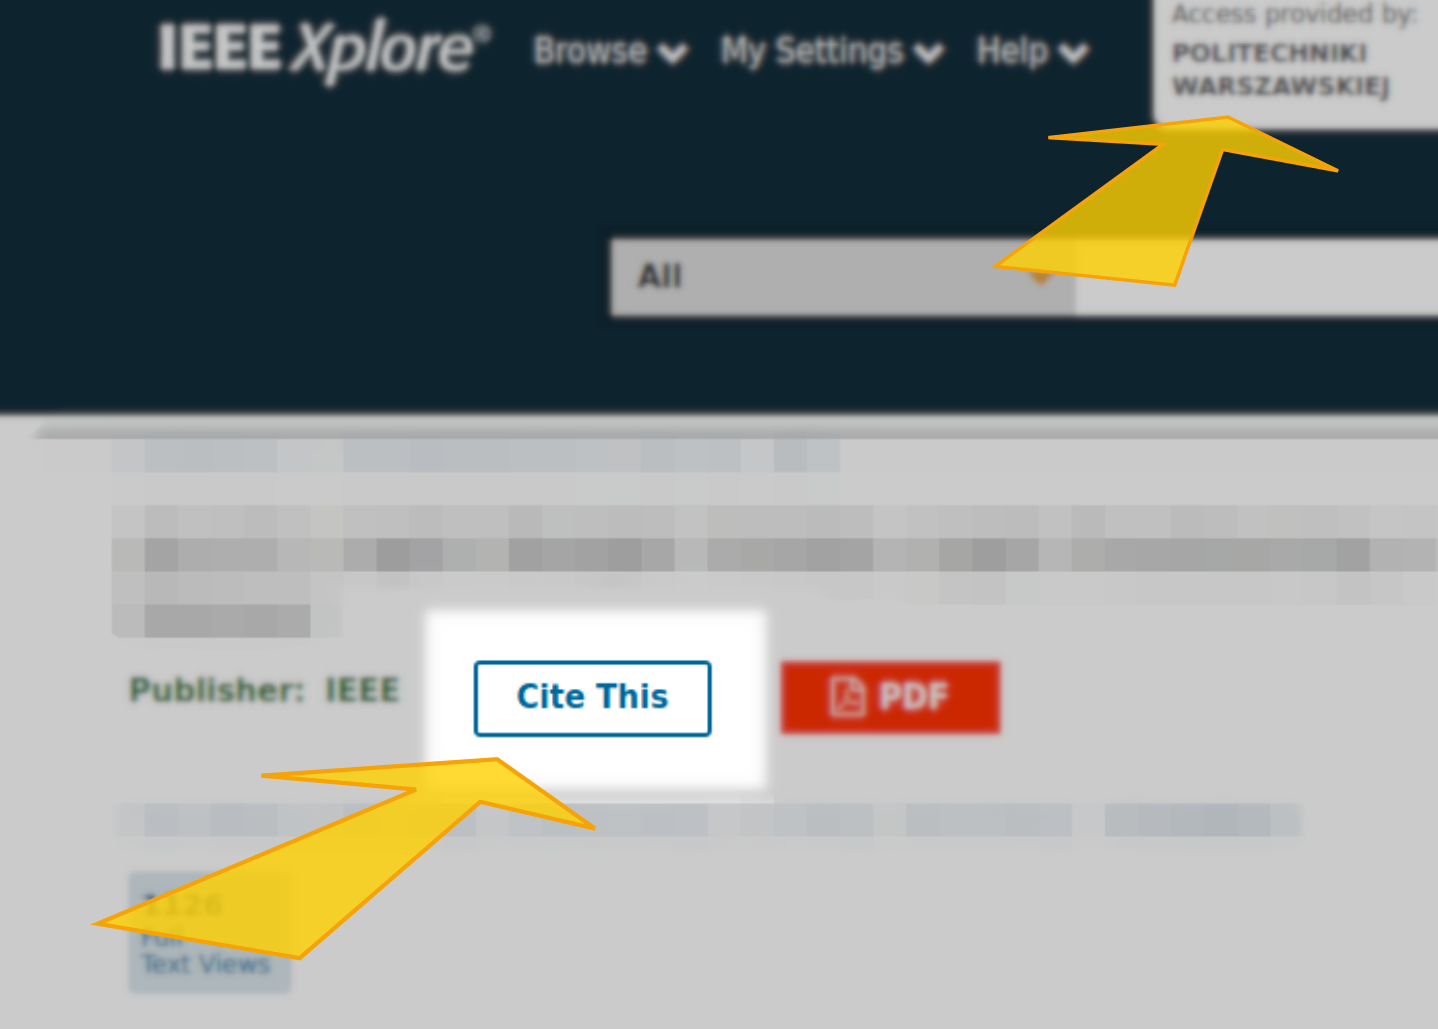
\includegraphics[width=16cm]{citethis.png} % rysunek o szerokości bezwzględnej
	\caption{Przykład możliwości pobrania noty bibliograficznej ze strony wydawcy}
	\label{rys:citethis}
\end{figure}

Ułatwieniem może być to, że serwisy takie jak IEEE Xplore pozwalają na pobranie cytowania w~postaci BibTeX. Nie do końca prawidłowo wypełniają i~używają pól ale mamy pewność, że składnia jest poprawna. Studenci i~pracownicy Politechniki Warszawskiej mają dostęp do tych zasobów za pośrednictwem \href{https://bg.pw.edu.pl/}{Biblioteki Głównej PW} -- znajdź na stronie odnośnik ,,Lista e-baz''. Z serwisu IEEE Xplore pobieramy cytowanie w~taki sposób, jak pokazane jest to na rysunku~\ref{rys:citethis}. Inne serwisy gromadzące publikacje zazwyczaj mają podobną funkcję.

\paragraph{Przykład 1.}
James Clerk Maxwell opublikował swe wiekopomne dzieło mając 35 lat~\cite{maxwell1865}. Maxwell zręcznie połączył znane wcześniej teorie i~nadał im nowe znaczenie ale pozostał teoretykiem. Musiały minąć dwie dekady zanim Heinrich Hertz wykazał, jakie praktyczne znaczenie ma fakt rozchodzenia się fal elektromagnetycznych~\cite{cichon1995}. Na tych fundamentach opierają się najnowsze osiągnięcia techniki wykorzystujące bezprzewodową transmisję danych, takie jak Internet Rzeczy~\cite{lncsevo}.

\paragraph{Przykład 2.} International Conference on Computational Problems of Electrical Engineering (CPEE) to coroczna konferencja współorganizowana przez IETiSIP a~skupiająca naukowców z~krajów ościennych Polski takich jak: Ukraina, Czechy, Słowacja. Jej lokalizacja zmienia się cyklicznie między tymi krajami. Na przykład w~roku 2018 CPEE odbyła się w~miejscowości Banská Štiavnica na Słowacji~\cite{cpee2018}.

\paragraph{Przykład 3.} W~Internecie Rzeczy (ang. \textit{Internet of Things}, IoT) jednym z~problemów jest zapewnienie odpowiedniego poziomu wiarygodności~\cite{truong2018}. Aktualnym tematem badawczym jest wykorzystanie metody łańcucha bloków (ang. \textit{Blockchain}) w~celu zwiększenia poziomu zaufania do systemu informatycznego~\cite{poirier2020}. Ma to szczególne znaczenie ze względu na rosnący udział urządzeń IoT w~incydentach bezpieczeństwa~\cite{nask2020}. Podstawą bezpieczeństwa we współczesnych systemach kryptograficznych jest generator liczb prawdziwie losowych (ang. \textit{True Random Number Generator}, TRNG), obecny w~niektórych typach procesorów~\cite{AN4230}.

\paragraph{Przykład 4.} Nota bibliograficzna nie może składać się wyłącznie z~adresu internetowego. Jak widać z~przedstawionych przykładów można w~literaturze umieścić praktycznie wszystko i~zrobić to w~sposób prawidłowy, to jest podając autora, tytuł i~inne pola noty bibliograficznej. Nie powołujemy się jednak na źródła wtórne, takie jak Wikipedia. Można za to przywołać nawet takie źródła jak zasoby bazodanowe i~repozytorium plików~\cite{szablon}.

%%%%%%%%%%%%%%%%%%%%%%%%%%%%%%%%%%%%%%%%%%%%%%%%
\section{Cytowania}
Cytowania nie są popularne w~naukach technicznych. Jednak przywołując czyjeś słowa trzeba cytat stosownie oznaczyć za pomocą cudzysłowów i~odniesienia do literatury.

Cytując \textbf{nie należy} korzystać ze znaku " dostępnego na klawiaturze, ponieważ nie jest to zgodne z~polską tradycją piśmienniczą. Cytowania tekstu standardowo robi się ,,recznie'', oznaczając cudzysłowy za pomocą podwójnych przecinków i~apostrofów. Jeszcze lepiej -- skorzystać z~poleceń jak poniżej.

Cytaty zagnieżdżone zrealizowane poleceniem \texttt{enquote}:
\enquote{\enquote{Daj, ać ja pobruczę, a~ty poczywaj}. To najstarsze zapisane po polsku zdanie, przekazane przez XIII-wiecznego, niemieckiego z~pochodzenia autora łacińskojęzycznej Księgi Henrykowskiej, w~dalekim od fonetycznej poprawności zapisie: \enquote{day, ut ia pobrusa, a~ti poziwai}}~\cite{wilamowski2017}.

Cytaty obcojęzyczne są możliwe za pomocą polecenia \texttt{foreignquote} dla języków zdefiniowanych w~nagłówku. Mikołaj Kopernik, przedstawiony na rysunku ze strony~\pageref{rys:kopernik}, jest autorem słów: \foreignquote{latin}{Iam quia demonstratum est, terram quoque globi formam habere, videndum arbitror, an etiam formam eius sequatur motus, et quem locum universitatis obtineat, sine quibus non est invenire certam apparentium in cœlo rationem}.

%%%%%%%%%%%%%%%%%%%%%%%%%%%%%%%%%%%%%%%%%%%%%%%%
\section{Kolory}
Zarządzenie nr 57/2016 JM Rektora PW definiuje kolory dla poszczególnych grup wydziałów:
\begin{itemize}
 \item Kolor ,,miętowy'' -- \colorbox{bud}{wydziały ,,budowlane'':}{\color{bud} Architektury, Geodezji i~Kartografii, Inżynierii Lądowej, Instalacji Budowlanych, Hydrotechniki i~Inżynierii Środowiska, Transportu.}
 \item Kolor ,,morelowy'' -- \colorbox{mech}{wydziały ,,mechaniczne'':}{\color{mech} Inżynierii Produkcji, Mechaniczny Energetyki i~Lotnictwa, Mechatroniki, Samochodów i~Maszyn Roboczych.}
 \item Kolor ,,słoneczny'' -- \colorbox{chem}{wydziały ,,chemiczne'':}{\color{chem} Chemiczny, Inżynierii Chemicznej i~Procesowej, Inżynierii Materiałowej.}
 \item Kolor ,,szafirowy'' -- \colorbox{elek}{wydziały ,,elektryczne'':}{\color{elek} Elektryczny, Elektroniki i~Technik Informacyjnych.}
 \item Kolor ,,śliwkowy,'' -- \colorbox{mfiz}{wydziały ,,matematyczno-fizyczne'':}{\color{mfiz} Fizyki, Matematyki i~Nauk Informacyjnych.}
 \item Kolor ,,wrzosowy'' -- \colorbox{multi}{wydziały ,,multidyscyplinarne'' oraz ,,społeczno-ekonomiczne'':}{\color{multi} Administracji i~Nauk Społecznych, Zarządzania, Budownictwa,~Mechaniki i~Petrochemii; Kolegium Nauk Ekonomicznych i~Społecznych.}
\end{itemize}

\subsection{Przykład zdefiniowanej palety kolorów}
Na rysunku~\ref{rys:colorsample} pokazana jest propozycja bardziej rozbudowanego zestawienia kolorów, zdefiniowana w~niniejszym szablonie. Podstawowa barwa Wydziału Elektrycznego, zgodnie z~obowiązującymi na PW zasadami dotyczącymi prac dyplomowych to \textcolor{EEBlue}{EEBlue}. Dodatkowo zdefiniowane są jej dwa odcienie:
\begin{itemize}
    \item ton jaśniejszy (ang. \textit{tint}) \textcolor{EEBlueLight}{EEBlueLight} (EEBlueLight),
    \item ton ciemniejszy (ang. \textit{shade}) \textcolor{EEBlueDark}{EEBlueDark}.
\end{itemize}
Odcienie i~barwa podstawowa są jednolite chromatycznie, czyli w~modelu HSV mają tę samą barwę ,,H''. Ton ciemniejszy ma mniejszą wartość (,,V'') a~ton jaśniejszy większą wartość (,,V'') i~mniejsze nasycenie (,,S''). Zaletą ich stosowania jest to, że te trzy tony bez problemu odróżnią osoby mające problemy z~rozpoznawaniem barw. 

% Rysunek przy użyciu tikz
\begin{figure}[!ht]
    \centering
	\resizebox*{0.618\linewidth}{!}{%
        \begin{tikzpicture}every node/.append style = {anchor=center}
            \filldraw[fill=EEBlue] (-0.5,-0.25) rectangle (10.5,8.75);
            \fill[EEBlueLight] (0,7.5) rectangle (10,8.5);
            % duża przerwa
            \fill[EEBlueDark] (0,5.5) rectangle (10,6.5);
            \fill[EEOrange] (0,4.25) rectangle (10,5.25);
            \fill[EETangerine] (0,3) rectangle (10,4);
            \fill[EEGold] (0,2) rectangle (10,3);
            \fill[EEAzure] (0,1) rectangle (10,2);
            \fill[EEUltramarine] (0,0) rectangle (10,1);
            \node at (5,7.90) {\large \textcolor{EEBlueDark}{EEBlueLight} \#e2ecf8};
            \node at (5,6.90) {\large \textcolor{EEBlueDark}{EEBlue} \#8ba5d3};
            \node at (5,5.90) {\large \textcolor{EEBlueLight}{EEBlueDark} \#45536a};
            \node at (5,4.65) {\large \textcolor{EEBlueDark}{EEOrange} \#f6a307};
            \node at (5,3.40) {\large \textcolor{EEBlueDark}{EETangerine} \#ff7700};
            \node at (5,2.40) {\large \textcolor{EEBlueDark}{EEGold} \#ffd100};
            \node at (5,1.40) {\large \textcolor{EEBlueLight}{EEAzure} \#0088ff};
            \node at (5,0.40) {\large \textcolor{EEBlueLight}{EEUltramarine} \#002eff};
        \end{tikzpicture}
	}
    \caption{Próbka zdefiniowanych kolorów}
    \label{rys:colorsample}
\end{figure}

Bladopomarańczowy kolor nazwany \textcolor{EEOrange}{EEOrange} jest dopełniającym dla podstawowego koloru wydziałowego EEBlue. Ton ten leży po przeciwnej stronie koła barw niż ton podstawowy a~więc tworzy z~nim silny kontrast. Może to dawać bardzo dobry lub bardzo kiepski efekt. Ponadto dla osób z~całkowitym daltonizmem te dwie barwy mogą być trudno odróżnialne. Dlatego warto rozważyć jej łączenie z~tonem jaśniejszym lub ciemniejszym barwy podstawowej.

Dodatkowo zdefiniowana jest tetrada barw uzupełniających, która w~połączeniu z~barwą podstawową lub jej odcieniami może dać dobry efekt wizualny. Te barwy to:
\begin{itemize}
    \item \colorbox{EETangerine}{mandarynkowy} -- \textcolor{EETangerine}{EETangerine} (EETangerine),
    \item \colorbox{EEGold}{złoty} --  \textcolor{EEGold}{EEGold} (EEGold),
    \item \colorbox{EEAzure}{lazurowy} --  \textcolor{EEAzure}{EEAzure} (EEAzure),
    \item \colorbox{EEUltramarine}{\textcolor{white}{ultramaryna}} --  \textcolor{EEUltramarine}{EEUltramarine} (EEUltramarine).
\end{itemize}
Barwy mandarynkowa i~złota mogą się dobrze kojarzyć z~barwami loga Wydziału Elektrycznego.

W pracy dyplomowej użycie barw powinno być bardzo ograniczone i~dobrze przemyślane. Kolory silnie kontrastowe, szczególnie ciepłe barwy pomarańczowo-żółte w~zestawieniu z~zimną barwą podstawową Wydziału Elektrycznego należy używać nadzwyczaj ostrożnie aby nie uzyskać niepoważnego, ,,choinkowego'' efektu.

%%%%%%%%%%%%%%%%%%%%%%%%%%%%%%%%%%%%%%%%%%%%%%%%
\section{Tabele}
Prostą tabelą, wprowadzoną ręcznie, jest tabela~\ref{tab:zjawiska}, która przedstawia kilka dat zjawisk astronomicznych. Tego rodzaju tabela wystarczy w~większości prac. Wygląd tabelaryczny uzyskuje się za pomocą otoczenia \texttt{tabular}. Sam wygląd tabelaryczny to jednak jeszcze nie jest tabela, tak jak zbiór komórek z~arkusza kalkulacyjnego nie jest tabelą, w~rozumieniu składu tekstu. Aby uzyskać tabelę należy \texttt{tabular} otoczyć za pomocą środowiska \texttt{table}. Wtedy taką tabelę można opatrzyć podpisem (\texttt{caption}) i~znacznikiem pozwalającym na odwołania do niej z~tekstu.

\begin{table}[h]
 \centering
  \begin{tabular}{p{2.5cm}c|l}
    Data        &   Godzina (UTC)   &   Zdarzenie\\\hline\hline
    2016-05-09  &   14:57           &   Tranzyt Merkurego\\\hline
    2017-08-11 --~2017-08-13  & --- &   Maksimum Perseidów \\\hline
    2018-07-27  &   20:22           &   Całkowite zaćmienie Księżyca\\\hline
    2019-08-24  &   17:04           &   Koniunkcja Wenus i~Mars w~odległości - 0°17`\\\hline
    2020-12-21  &   16:00           &   Koniunkcja Jowisz i~Saturn w~odległości 0°06`
  \end{tabular}
 \caption{\label{tab:zjawiska}Wybrane zjawiska astronomiczne z~lat 2016-2020}
\end{table}

Podobnie jak dla rysunków tak i~tabelom można wskazać posadowienie za pomocą oznaczeń literowych (h, b, t) i~wykrzyknika. Liczbę kolumn i~ułożenie w~nich tekstu określa się jako argumenty polecenia \texttt{tabular}:
\begin{itemize}
    \item l -- dosunięcie do lewej,
    \item r -- dosunięcie do prawej,
    \item c -- centrowanie,
    \item p -- styl akapitowy z~szerokością określoną parametrem.
\end{itemize}
Jeśli kolumny mają być oddzielone pionowymi liniami to między odpowiednimi literami powinna pojawić się pionowa kreska ,,|''.

W kolejnych liniach treści z~poszczególnych kolumn oddziela się znakiem ,,\&''. Wiersz tabeli kończy się {\LaTeX}owym znakiem nowego wiersza czyli podwójnym ukośnikiem: ,,\textbackslash\textbackslash''. Za nim można wstawić polecenie oznaczające narysowanie linii \texttt{\textbackslash{}hline}, która oddzieli dany wiersz tabeli od kolejnych. Można też zrobić podwójną linię (\texttt{\textbackslash{}hline\textbackslash{}hline}) w~celu odcięcia danego wiersza, na przykład nagłówka, od następnego za pomocą wąskiej, pustej przestrzeni.

Tabele są prawdopodobnie najtrudniejszym elementem do wprowadzenia w~\LaTeX{u} ze względu na nagromadzenie znaczników. Dlatego warto rozważyć edytowanie pracy lub przynajmniej tabel za pomocą dedykowanego edytora takiego jak Kile\footnote{\href{https://kile.sourceforge.io/}{<https://kile.sourceforge.io/>}}. Zrzut ekranu pokazujący edycję tabeli w~tym programie pokazany jest na rysunku~\ref{rys:kile}.
Bardziej skomplikowana tabela~\ref{tab:kolorowatabela} została przygotowana w~Kile, skopiowana tutaj i~później zmodyfikowana.

\begin{figure}[!t]
	\centering 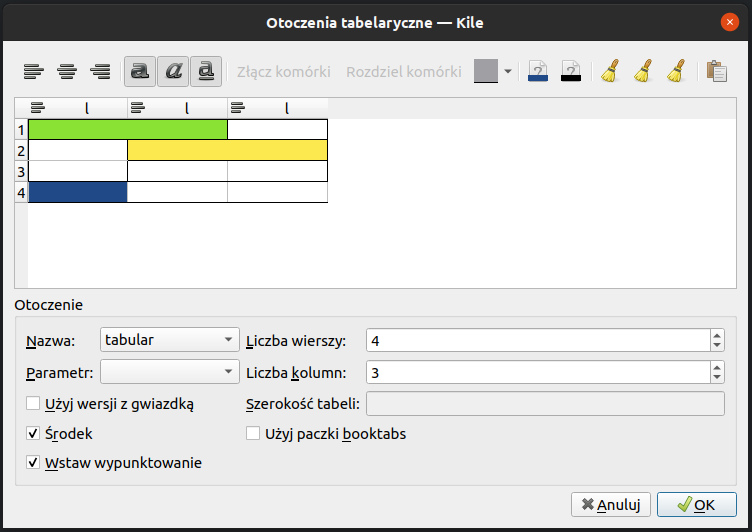
\includegraphics[height=0.25\textheight]{kile.png} % rysunek o wysokości 1/4 wysokości tekstu na stronie
	\caption{Wykorzystanie programu Kile do edycji tabeli}
	\label{rys:kile}
\end{figure}

{%
\newcommand{\mc}[3]{\multicolumn{#1}{#2}{#3}}
 \begin{table}[!ht]
 \centering
  \begin{tabular}{lll}\cline{1-1}\cline{3-3}
   \rowcolor{EEBlue}
   \mc{2}{|l|}{×} & \mc{1}{l|}{×}\\\hline\hline
   \mc{1}{|l|}{×} & \mc{2}{>{\columncolor{EEBlueDark}}l|}{\textcolor{EEGold}{×}}\\\cline{2-3}
   \rowcolor{EEBlueLight}
   \mc{1}{|l|}{×} & × & \mc{1}{l|}{×}\\\hline
   \rowcolor{EETangerine}
   × & × & ×\\\hline
  \end{tabular}
  \caption{Bardziej skomplikowana tabelka}
  \label{tab:kolorowatabela}
 \end{table}
}%


%%%%%%%%%%%%%%%%%%%%%%%%%%%%%%%%%%%%%%%%%%%%%%%%
\section{Wzory}
Jakość aplikacji do edycji tekstu najłatwiej poznać po typografii wzorów. W~tym obszarze prawdopodobnie nie ma lepszego narzędzia niż \LaTeX{}. Wzory zapisywane są za pomocą zbioru poleceń. Tego samego zestawu znaczników do zapisu wzorów używa Wikipedia. Proste, bardziej popularne symbole matematyczne i~oznaczenia po pewnym czasie po prostu się pamięta. Jeśli chcemy uzyskać bardziej skomplikowane wzory lub użyć mniej popularnych symboli to warto sięgnąć po dokumentację dostępną na przykład na stronach Overleaf\footnote{\href{https://www.overleaf.com/learn/latex/Mathematical_expressions}{<Overleaf -- Mathematical expressions>}}. Można też wspomóc się zewnętrzną aplikacją taką jak na przykład Kile. Alternatywnie można skorzystać z~edytorów równań dostępnych online, takich jak:
\begin{itemize}
    \item \href{https://latex.codecogs.com/eqneditor/editor.php}{CodeCogs}
    \item \href{https://www.latex4technics.com/}{Latex4technics}
\end{itemize}
Ich zaletą jest niemal natychmiastowe pokazywanie efektu. Poniżej znajduje się kilka przykładów zapisania wzorów.

\subsection{André-Marie Ampère}
André-Marie Ampère urodził się 20 stycznia 1775 roku. Był francuskim fizykiem i~matematykiem, pionierem w~zakresie badań nad elektromagnetyzmem. W~kształceniu od wczesnych lat wspierał go ojciec, z~którego znacznej biblioteki Ampère swobodnie korzystał. Chociaż nie otrzymał formalnego wykształcenia to uzyskał wysoką renomę jako nauczyciel i~niezależny badacz. Dzięki temu został profesorem matematyki w~École polytechnique. Następnie kierował katedrą fizyki w~Collège de France. Został członkiem Francuskiej Akademii Nauk. Jego portret pokazany jest na rysunku~\ref{rys:ampere}. Ampère zmarł 10 czerwca 1836 roku, która to data została później przyjęta przez Stowarzyszenie Elektryków Polskich jako ,,Międzynarodowy Dzień Elektryka''.

\begin{figure}[!hb]
	\centering 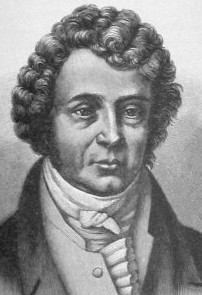
\includegraphics[width=0.25\linewidth]{Ampere.jpg}
	\caption{André Marie Ampère}
	\label{rys:ampere}
\end{figure}

\begin{equation}
    \oint \vec{H} d\vec{l} = \int\limits_{S} \vec{J} \cdot d \vec{a} = I
\end{equation}

\begin{equation}
    \nabla \times \vec{H} = \vec{J}
\end{equation}

\subsection{Michael Faraday}
Michael Faraday urodził się 22 września 1791 roku w~niezamożnej rodzinie i~otrzymał jedynie wykształcenie podstawowe. W~dużej mierze był samoukiem ale już jako kilkunastolatek dał się poznać jako człowiek utalentowany i~otrzymał wsparcie ze strony ludzi kultury, i~nauki. Wniósł fundamentalny wkład do badań nad elektromagnetyzmem i~elektrochemią. Odkrył zjawisko indukcji elektromagnetycznej i~zbudował pierwszy silnik elektryczny. Badał oddziaływanie światła z~materią i~między innymi odkrył zjawisko magnetooptyczne. Wykonane przez niego koloidalne złoto nadal jest aktywne. Zajmując się chemią odkrył benzen. Został członkiem Royal Institute oraz wielu towarzystw naukowych w~innych krajach. Mimo licznych sukcesów i~możliwości unikał zyskiwania stanowisk i~tytułów. Faraday Zmarł w~roku 1867. Jego portret pokazany jest na rysunku~\ref{rys:faraday}.

\begin{figure}[!ht]
	\centering 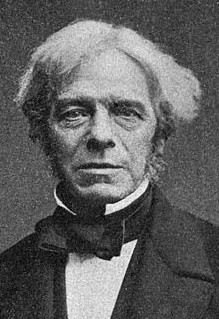
\includegraphics[width=0.25\linewidth]{Faraday.jpg}
	\caption{Michael Faraday}
	\label{rys:faraday}
\end{figure}

\begin{equation*}
    \Phi_B = \iint\limits_{\sum (t)} \pmb{B}(t) \cdot d\pmb{A}
\end{equation*}

\begin{equation}
    \mathcal{E} = -\frac{d\Phi_B}{dt}
\end{equation}

 \begin{equation}
     \nabla \times \pmb{E} = - \frac{\partial \pmb{B}}{\partial t}
 \end{equation}


\subsection{Georg Simon Ohm}
Georg Simon Ohm urodził się 16 marca 1789 roku w~Erlangen. We wczesnych latach życia większość wiedzy i~wykształcenia otrzymał od własnego ojca, samouka. W~wieku 22 lat uzyskał doktorat z~matematyki na Uniwersytecie w~Erlangen, gdzie przez krótki czas również pracował. W~latach 1833-1849 był profesorem Politechniki w~Norymberdze a~następnie Uniwersytetu w~Monachium. Sformułował prawo opisujące zależność między prądem a~napięciem $U=R \cdot I$. Zmarł w~roku 1854 w~Monachium. Jego portret pokazany jest na rysunku~\ref{rys:ohm}.

\begin{equation}
    R = \frac{U}{I}
\end{equation}

\begin{figure}[!h]
	\centering 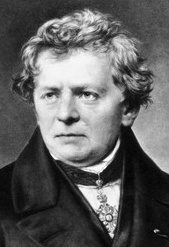
\includegraphics[width=0.25\linewidth]{Ohm.jpg}
	\caption{Georg Simon Ohm}
	\label{rys:ohm}
\end{figure}

\begin{equation*}
    \vec{J} = nq \vec{v_d} =  \frac{nq^2 \tau}{m} \vec{E} = nq \mu \vec{E}    
\end{equation*}
 
Wzór~\ref{eq:ohm} wiąże gęstość prądu $\pmb{J}$ z~natężeniem pola elektrycznego $\pmb{E}$ w~przewodniku.
 
\begin{equation}
    \pmb{J} = \sigma \pmb{E}
    \label{eq:ohm}
\end{equation}


\subsection{James Clerk Maxwell}
James Clerk Maxwell urodził się 13 czerwca 1831 roku w~Edynburgu, w~szkockiej rodzinie szlacheckiej. Uczęszczał do Akademii Edynburskiej a~następnie, jako szesnastolatek na Uniwersystet w~Edynburgu. W~roku 1850 przeniósł się na Uniwersytet w~Cambridge. Mając lat 25 zostawił Cambridge by zostać profesorem na Uniwersytecie w~Aberdeen. Po przekształceniach na uczelni musiał opuścić Aberdeen i~w~roku 1860 podjął pracę w~Kolegium Królewskim w~Londynie, gdzie regularnie spotykał się z~Faradayem. Jego słynne równania, które zunifikowały pole magnetyczne i~elektryczne a~tym samym zmieniły sposób myślenia o~fizyce, zostały zaprezentowane światu w~roku 1865~\cite{maxwell1865}. We współczesnej formie przedstawione są wzorami~\ref{eq:maxwell1}--\ref{eq:maxwell4}. Maxwell zmarł mając lat 48, w~roku 1879. Portret Maxwella jest pokazany na rysunku~\ref{rys:maxwell}.

\begin{figure}[!t]
	\centering 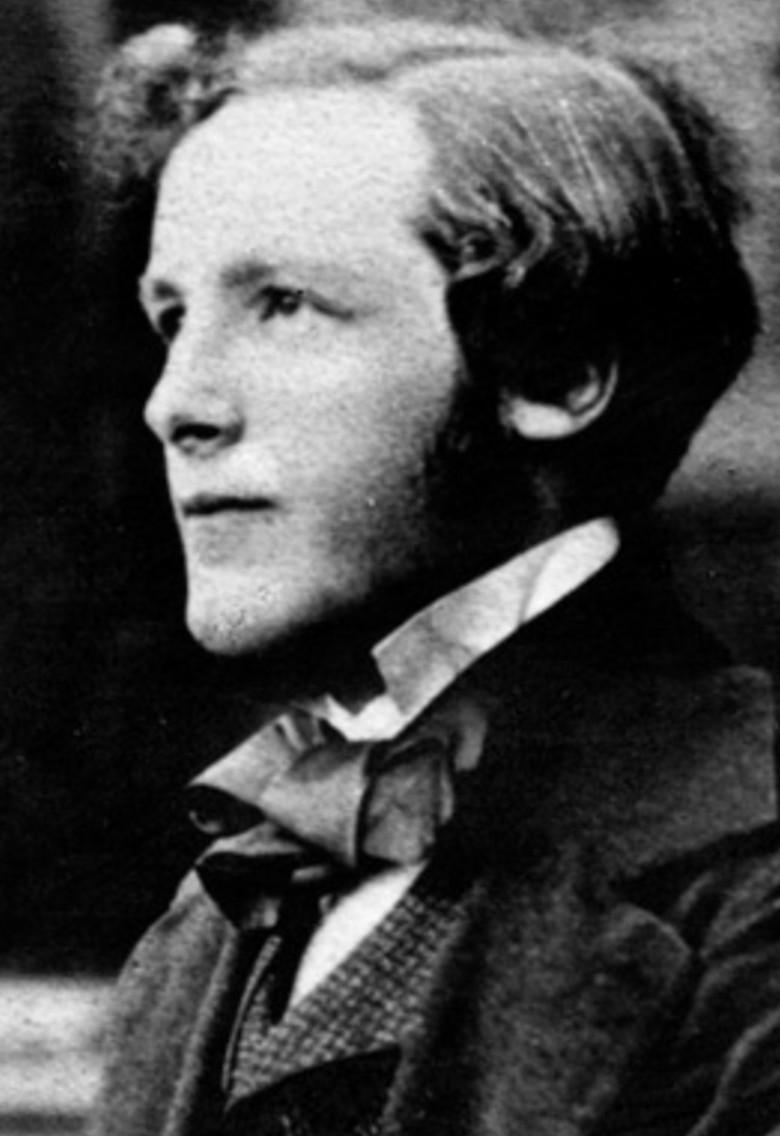
\includegraphics[width=0.25\linewidth]{Maxwell.jpg}
	\caption{James Clerk Maxwell}
	\label{rys:maxwell}
\end{figure}

\begin{align}
\oiint\nolimits_{\partial \Omega} \pmb{E} \cdot \mathrm{d}\pmb{S} &= \frac{1}{\varepsilon_0} \iiint\nolimits_\Omega \rho \, \mathrm{d}V &  \nabla \cdot \pmb{E} &= \frac {\rho} {\varepsilon_0} \label{eq:maxwell1} \\
\oiint\nolimits_{\partial \Omega} \pmb{B} \cdot \mathrm{d}\pmb{S} &= 0 & \nabla \cdot \pmb{B} &= 0 \label{eq:maxwell2} \\
\oint\nolimits_{\partial \Sigma} \pmb{E} \cdot \mathrm{d}\boldsymbol{\ell} &= -\frac{\mathrm{d}}{\mathrm{d}t}\iint\nolimits_{\Sigma}\pmb{B}\cdot\mathrm{d}\pmb{S} & \nabla \times \pmb{E} &= -\frac{\partial \pmb{B}}{\partial t} \label{eq:maxwell3} \\
\oint\nolimits_{\partial \Sigma} \pmb{B} \cdot \mathrm{d}\boldsymbol{\ell} &= \mu_0 \iint\nolimits_{\Sigma} \pmb{J} \cdot \mathrm{d}\pmb{S} + \mu_0 \varepsilon_0 \frac{\mathrm{d}}{\mathrm{d}t} \iint\nolimits_{\Sigma} \pmb{E} \cdot \mathrm{d}\pmb{S} & \nabla \times \pmb{B} &= \mu_0\left(\pmb{J} + \varepsilon_0 \frac{\partial \pmb{E}} {\partial t} \right) \label{eq:maxwell4}
\end{align}


\subsection{Jeszcze kilka przypadkowo wybranych wzorów}
Równania normalnie otrzymują kolejne numery. Jeśli nie chcemy aby dane równanie było numerowane, bo jest na przykład zbyt mało ważne, to używamy gwiazdki przy oznaczeniu używanego otoczenia (czyli zazwyczaj equation). Należy pamiętać, że otoczenie otwarte z~gwiazdką musi być również zamknięte z~gwiazdką.
\begin{equation*}
    r = \sqrt{r_x^2 + r_y^2}
\end{equation*}

\begin{equation}
    \frac{dx}{dx} = 1
\end{equation}

\begin{equation}
    \frac{d}{dx} \ln x = \frac{1}{x}
\end{equation}

\begin{equation}
    y = \varphi  (y^\prime)x + \psi(y^\prime)
\end{equation}

\begin{equation}
    f(t) = \frac{1}{\pi} \int\limits_0^\infty \mathrm{d} \omega \,\int\limits_{-\infty}^{+\infty} f(\tau)\, \cos \omega (t-\tau)  \mathrm{d}\tau
\end{equation}

\[
\mathfrak{F}^{-1}\left(\mathfrak{F} \left[ f\left(t \right ) \right ] \right ) = f \left(t \right )
\qquad \textup{oraz} \qquad
\mathfrak{F}\left(\mathfrak{F}^{-1} \left[ F\left(j\omega \right ) \right ] \right ) = F \left(j\omega \right )
\]

\begin{equation*}
    x \oplus y = \neg (x \equiv y) = (x \vee y) \wedge (\neg x \vee \neg y) = (x \wedge \neg y) \vee (\neg x \wedge y)
\end{equation*}

\begin{equation*}
    \sum \frac{Q}{T} = 0
\end{equation*}

\begin{equation}
    \oint \frac{dQ}{T} = 0
\end{equation}

\begin{equation}
    \pmb{a} = \lim\limits_{\Delta t \to 0} \frac{\Delta \pmb{v}}{\Delta t} = \frac{d\pmb{v}}{dt}
\end{equation}

\begin{equation}
K = m\,c^2 - m_0\,c^2 
 = m_0\,c^2 \left(
  \frac{1}{ \sqrt{1 - \left( \frac{v}{c} \right)^2 } } -1 
 \right)
\end{equation}

\begin{equation}
    \frac{\partial^2 y}{\partial x^2} = \frac{\mu}{F} \; \frac{\partial^2 y}{\partial t^2}
\end{equation}

\begin{equation}
    e^{\pm i\theta} = \cos \theta \pm i~\sin\theta
\end{equation}

\begin{equation}
    U(M) = \lim\limits_{R\to 0} \iiint\limits_{G-K}\frac{\rho(P)}{r}dG
\end{equation}

\begin{equation*}
    \left| \, \int\limits_{C_R} \frac{dz}{\left( 1+z^2 \right )^3} \, \right| \leqslant \sup\limits_{z \in C_R} \frac{1}{\left| 1+z^2 \right|^3} \; \pi R
\end{equation*}

W otoczeniu \texttt{align} można umieścić kilka wzorów jeden pod drugim oddzielając je znakiem nowego wiersza, czyli podwójnym ukośnikiem: \texttt{\textbackslash{}\textbackslash{}}. Wzory te poukładają się elegancko jeden pod drugim, jeśli w~każdej linii umieścimy jeden lub więcej znaków \&. Ważne, żeby w~każdej linii znak \texttt{\&} wystąpił tyle samo razy, gdyż wskazuje on miejsce wyrównania równań w~kolumnie.

\begin{align}
    g & = \frac{v^2}{R+h} \\
    v & = \sqrt{ \left( R+h \right) g }
\end{align}

\begin{align}
 y(t) = A_0 
 +& A_1 \sin \omega t + 
    A_2 \sin 2 \omega t + 
    A_3 \sin 3 \omega t + \ldots + \nonumber \\
 +& B_1 \cos \omega t + 
    B_2 \cos 2 \omega t + 
    B_1 \cos 3 \omega t + \ldots
\end{align}

\begin{align}
 \nu^\prime  &= \frac{\left(vt / \lambda \right) + \left( v_0t / \lambda \right)}{t} = \nonumber\\
            &= \frac{v + v_0}{\lambda} = \nonumber\\
            &= \frac{v + v_0}{v / \nu} = \nonumber\\
            &= \nu \frac{v+v_0}{v} = \nonumber\\
            &= \nu \left( 1 + \frac{v_0}{v} \right)
\end{align}

Można wygenerować zdecydowanie bardziej skomplikowane wzory. Otoczenie \texttt{gather} pozwala na łączenie na przykład macierzy ze ,,zwykłymi'' wzorami.

\begin{gather}
 \begin{bmatrix} \Phi_{11} & \Phi_{12} \\ \Phi_{21} & \Phi_{22} \end{bmatrix}
 =
 \frac{1}{\det(X)}
  \begin{bmatrix}
   X_{22} Y_{11} - X_{12} Y_{21} &
   X_{22} Y_{12} - X_{12} Y_{22} \\
   X_{11} Y_{21} - X_{21} Y_{11} &
   X_{11} Y_{22} - X_{21} Y_{12} 
   \end{bmatrix}
\end{gather}

\begin{gather}
a \times b = -b \times a~= 
\begin{vmatrix}
\pmb{i}    &     \pmb{j}      &      \pmb{k}    \\
a_x        &     a_y          &      a_z        \\
b_x        &     b_y          &      b_z        
\end{vmatrix}
= \left(a_y b_z - b_y a_z \right)\pmb{i} 
+ \left(a_z b_x - b_z a_x \right)\pmb{j} 
+ \left(a_x b_y - b_x a_y \right)\pmb{k} 
\end{gather}

% Na Wydziale Elektrycznym wzorów chemicznych raczej nie potrzebujemy zbyt często a~te kilka przypadków da się zapisać jako zwykłe równania.
% Gdyby jednak ktoś bardzo chciał to można odkomentować linijkę z~pliku cls:
%\RequirePackage[version=4]{mhchem}
% a~wtedy zadziałają poniższe makra:
%\ce{3H2O} \\
%\ce{1/2H2O} \\
%\ce{AgCl2-} \\
%\ce{H2_{(aq)}}

\section{Kody źródłowe}
Do umieszczania kodów źródłowych w~szablonie wykorzystany jest pakiet \texttt{listings}. Została przygotowana propozycja wyglądu listingów oparta o~prezentowane wcześniej kolory. Ustawienia można zmienić w~pliku \texttt{cls}. Poniżej znajduje się kilka przykładów wykorzystania wspomnianego pakietu. Więcej informacji można znaleźć na przykład w~dokumentacji Overleaf\footnote{\href{https://www.overleaf.com/learn/latex/code_listing}{<Overleaf -- Code listing>}}

Kod źródłowy można umieścić bezpośrednio w~pliku tex, tak jak poniższy przykład z~listingu~\ref{lst:hellopy}. Zauważ niezbyt fortunne przejście na nową stronę, zakłócone przez przypis dolny, czego niestety \LaTeX{} nie jest w~stanie poprawić. Należałoby tu dopisać coś więcej by ,,przepchnąć'' kod na kolejną stronę.

\begin{lstlisting}[language=Python,
    caption={Prosty program w~języku Python},
    label={lst:hellopy}]
#!/usr/bin/env python
# -*- coding: utf-8 -*-
"""Simple world of hello.
"""

import sys

def main():
    """The one and only function"""
    fib = lambda n: reduce(lambda x, n: [x[1], x[0]+x[1]], range(n), [0, 1])[0]
    try:
        print(fib(int(sys.argv[1])))
    except:
        print("Hello World!")

if __name__ == "__main__":
    main()
\end{lstlisting}

Zauważ automatyczne kolorowanie składni i~numerowanie linii. Spójna kolorystyka kodów w~różnych językach może być pożądana albo wręcz przeciwnie. Dlatego można rozważyć jakąś, niewielką, lokalną zmianę stylu tak, jak w~poniższym przykładzie. Przykład kodu źródłowego w~innym języku (tutaj: C) jest pokazany w~listingu~\ref{lst:helloC}. 

\begin{lstlisting}[language=C,
    backgroundcolor=\color{EEGold!5!white},
    caption={Prosty program w~języku C},
    label={lst:helloC}]
#include <stdlib.h>
#include <stdio.h>
/* 
Simple world of hello.
*/

int main(int argc, char **argv) {
	printf("Hello World!\n");
	return EXIT_SUCCESS;
}
\end{lstlisting}

Kod źródłowy można też trzymać w~zewnętrznym pliku i~załączać go do dokumentu dynamicznie, tak jak ma to miejsce w~przypadku listingu~\ref{lst:Keccak}. Można wskazać zakres linii, które powinny pojawić się w~dokumencie. Jednak wtedy zapewne warto pamiętać o~ustawieniu numeru pierwszej linii aby numeracja w~dokumencie zgadzała się z~faktycznym numerem linii w~pliku. Listing~\ref{lst:Keccak} ma automatycznie ustawiany podpis na podstawie nazwy pliku. W~pewnych sytuacjach może być to wygodniejsze niż ręczne wprowadzanie nazwy.

\lstinputlisting[language=C,
    firstnumber=31,
    firstline=31,
    lastline=50,
    caption=\lstname,
    label={lst:Keccak}]{Keccak-inplace32BI.c}

\section{Ostatnie drobiazgi}
Kilka ostatnich uwag odnośnie używania szablonu i~\LaTeX{a}.

\subsection{Podstawowe style tekstu}
W przykładowym dokumencie pojawiło się modyfikowanie wyglądu liter za pomocą kilku metod. Tu dla porządku zostaną one zebrane na jednej liście z~przykładami użycia:
\begin{itemize}
    \item \textbf{tekst wytłuszczony},
    \item \textit{tekst pochylony},
    \item \texttt{tekst maszynowy},
    \item \underline{tekst podkreślony}
    \item tekst \emph{wyróżniony} \textbf{odmiennym \emph{stylem}}, \textit{w zależności \emph{od sytuacji}} -- \emph{jest to \textbf{rozwiązanie} \textit{uniwersalne}}.
\end{itemize}

\subsection{Wiszące znaki}
W polskiej tradycji piśmienniczej samotne literki nie powinny występować na końcu linii. Aby połączyć taką literę z~następującym po nim słowem należy użyć znaku tyldy \keys{\textasciitilde{}}. Dotyczyć to może liter takich jak: a, i, o, u, w, z. Problem ten może dotyczyć też wielkich liter rozpoczynających zdania, o czym czasem zdarza się zapomnieć.


Pod koniec pisania pracy dobrze jest skorzystać z~opcji ,,znajdź i~zamień'' by wymienić wszystkie ciągi znaków \keys{\SPACE, znak, \SPACE} na \keys{\SPACE, znak, \textasciitilde{}}.

W~tym tekście zostało to zrobione.

\subsection{Wypunktowania}
\LaTeX{} ma duże możliwości jeśli chodzi o~formatowanie wypunktowań. Jednak zgodnie z~obowiązującymi na PW zaleceniami można stosować tylko dwa rodzaje punktorów:
\begin{itemize}
    \item standardową ,,kropkę'',
    \item[--] myślnik.
\end{itemize}
Zatem nie można używać wypunktowań numerycznych, list opisowych i~tak dalej.


\subsection{Dywiz a~myślnik}
Podejście do typografii w~\LaTeX{u} jest profesjonalne co wiąże się też z~dbałością o~rozróżnienie różnych rodzajów ,,myślników'':
\begin{itemize}
    \item pojedynczy znak minus ,,-'' to dywiz, stosowany do:
    \begin{itemize}
        \item przenoszenia wyrazów do nowej linii; uwaga: nie robimy tego ręcznie!
        \item łączenia słów (na przykład: Golub-Dobrzyń).
    \end{itemize}
    \item dwa znaki minus obok siebie ,,-{}-'' % tu celowo oddzielone, żeby się nie połączyły
    to ,,prawdziwy'' myślnik (--) o~wyraźnie większej długości od dywizu -- można go stosować w~zdaniach złożonych, oddzielając spacjami od sąsiadujących z~nim wyrazów,
    \item trzy znaki minus obok siebie praktycznie nie wystąpią w~pracach technicznych a~służą do oznaczania dialogów. --- Serio? --- Ano tak.
\end{itemize}

\subsection{Akronimy i~symbole}
Zgodnie z~obowiązującym Zarządzeniem pod koniec pracy znajduje się lista symboli i~akronimów pod nazwą ,,Wykaz symboli i~skrótów''. Na liście wystąpią tylko te akronimy, które faktycznie zostaną użyte w~tekście, za pomocą jednej z~pokazanych niżej metod. Jeśli żaden akronim lub symbol w~tekście nie wystąpi, w~sensie użycia odwołania za pomocą odpowiedniego polecenia, to generowanie strony z~listą akronimów zostanie pominięte. Większość prac do tej pory była pozbawiona tego dodatku.

Szablon używa pakietu \texttt{glossaries} do zarządzania akronimami i~symbolami. Listę tych elementów należy przygotować w~pliku \href{./glossary.tex}{glossary.tex}, zgodnie z~pokazanym tam szablonem. Aby w~pracy pojawiła się lista akronimów należy użyć polecenia:

\begin{lstlisting}[language=bash,
    numbers=none,
    caption=Wygenerowanie listy skrótów i~symboli,
    label={lst:gloss}]
makeglossaries [nazwa pliku podstawowego bez rozszerzenia tex]
\end{lstlisting}

Pierwsze użycie akronimu w~tekście jest rozpoznawane automatycznie i~pojawia się on w~pełnej oraz skróconej formie: \gls{CPEE}. Kolejnymi razy prezentuje się już tylko wersja skrócona, chociaż oba wywołania w~\LaTeX{u} wyglądają tak samo: \gls{CPEE}. Dzięki temu nie trzeba się zastanawiać, czy dany akronim został wcześniej pokazany w~pełnej formie, czy też jeszcze nie.

Można też samodzielnie wybrać jaką formę ma przybrać akronim w~tekście, co nie wpływa na rozpoznawanie pierwszego użycia skrótu:
\begin{itemize}
    \item krótkiej: \acrshort{IEEE}, \acrshort{PW}, \acrshort{IETiSIP},
    \item długiej: \acrlong{IEEE}, \acrlong{PW}, \acrlong{IETiSIP},
    \item pełnej: \acrfull{IEEE}, \acrfull{PW}, \acrfull{IETiSIP}.
\end{itemize}

Chociaż na powyższej liście występuje \gls{PW} to tutaj akronim jest traktowany jak pojawiający się po raz pierwszy. Dopiero kolejne użycie daje inny efekt: \gls{PW}.

W Overleaf wykorzystanie wykazu symboli matematycznych okazuje się sprawiać problemy -- indeks nie odświeża się. Dlatego w~pliku~\href{./EE-dyplom.cls}{EE-dyplom.cls} zakomentowana jest linia generująca listę symboli:
\begin{lstlisting}[language=TeX,
    numbers=none,
    caption=EE-dyplom.cls,
    label={lst:EE-dyplom}]
%    \printglossary[type=\acronymtype,title={}] % nie w Overleaf
%    \printglossary[type=symbols,title={}] % nie w Overleaf
\end{lstlisting}
Po pobraniu szablonu i~kompilacji lokalnej z~użyciem metody przedstawionej niżej, nie ma tego problemu i~linię można odkomentować, aby uzyskać ładną listę symboli.

Chcąc kompilować w~Overleaf a~zarazem mieć listę symboli, to niestety trzeba stworzyć ją ręcznie w~pliku \href{./symbols.tex}{symbols.tex}. Plik może zostać pusty ale musi istnieć.

Przykład użycia symbolu natężenia prądu elektrycznego~\gls{symb:I}. Jedną z~ciekawszych liczb jest~\gls{symb:Pi}. Tak użyte symbole przy prawidłowej kompilacji pliku \texttt{PDF} znajdą się na indeksowanej liście a~więc będzie można znaleźć miejsca ich użycia w~pracy. Oczywiście to indeksowanie zadziała tylko wtedy, gdy odwołamy się do symbolu w~przedstawiony sposób.

\subsection{Ozdobniki graficzne w~opisie oprogramowania}
Szablon wczytuje pakiet pozwalający na wyróżnienie w~tekście informacji o~skrótach klawiszowych, poruszaniu się po menu programu i~ścieżki plików. Oczywiście nie ma konieczności korzystania z~tego dodatku, jeśli ktoś nie uważa go za potrzebny.

W tekście można wyróżnić skróty klawiszowe, takie jak na przykład: \keys{\Alt, F4}, \keys{\ctrl, \Alt, \del}.
\begin{itemize}
    \item \keys{A, a, B, b, C, c, 1, 2, 3, PgUp}
    \item \keys{\Space} \keys{\SPACE}
    \item \keys{\backspace} \keys{\del} \keys{\backdel}
    \item \keys{\return} \keys{\enter}
    \item \keys{\shift} \keys{\capslock}
    \item \keys{\ctrl} \keys{\Alt} \keys{\AltGr}
    \item \keys{\tab}
    \item \keys{\esc} \keys{\oldesc}
    \item \keys{\winmenu}
    \item \keys{\arrowkey{^}} \keys{\arrowkeyup}
    \item \keys{\arrowkey{v}} \keys{\arrowkeydown}
    \item \keys{\arrowkey{>}} \keys{\arrowkeyright}
    \item \keys{\arrowkey{<}} \keys{\arrowkeyleft}
\end{itemize}

Jeśli opisujemy poruszanie się po menu to również można użyć ozdobnika graficznego: \menu{View > Zoom > Zoom in}.

Podobne rozwiązanie jest dla ścieżek katalogów: \directory{etc / apache2 / mods-available}.

\subsection{Puste miejsca}
Inne programy często mają problem z~prawidłowym wypełnieniem strony i~zostawiają na dole zbyt dużo pustego miejsca. Mają tę trudność głównie ze względu na problematyczne rozmieszczenie rysunków, tabel i~innych elementów graficznych. \LaTeX{} dobrze wypełnia przestrzenie stron i~zostawia na dole pustą przestrzeń tylko w~szczególnych, uzasadnionych przypadkach.

W \LaTeX nie ma problemu z~podwójnymi  czy wielokrotnymi      spacjami w~pliku \texttt{.tex}. Kompilator i~tak oblicza wielkość światła międzywyrazowego, by jak najlepiej ułożyć tekst na stronie. Stara się przy tym uniknąć nieprzyjemnych efektów graficznych takich jak ,,kanaliki''.

Strona tuż przed początkiem nowego rozdziału może zostać całkiem pusta i~nawet nie będzie mieć numeracji u~dołu. Jest to jak najbardziej prawidłowe, gdyż rozdziały mają zaczynać się od strony nieparzystej a~więc od strony prawej w~druku dwustronnym. Stron bez tekstu nie numeruje się, chociaż są one liczone.

\subsection{Kompilowanie lokalnie}
Darmowy dostęp do Overleaf zapewnia czas każdej kompilacji nie dłuższy niż 1 minuta. W~przypadku skomplikowanej pracy czas ten może zostać przekroczony i~wówczas Overleaf nie wygeneruje pliku wynikowego. Dlatego warto rozważyć pobranie szablonu na własny komputer z~zainstalowanym \XeLaTeX{em}. Kompilacja może wówczas wyglądać tak, jak na listingu~\ref{lst:kompilacja}.

\begin{lstlisting}[language=bash,
    caption={Kompilacja pracy dyplomowej lokalnie},
    label={lst:kompilacja}]
xelatex EE-dyplom && biber EE-dyplom && makeglossaries EE-dyplom && xelatex EE-dyplom && xelatex EE-dyplom
\end{lstlisting}

Polecenie \textbf{xelatex} można zastąpić przez \textbf{pdflatex} ale nie jest to zalecane.
